%\documentclass[10pt]{letter}
%\usepackage[utf8]{inputenc}

%%%%%%%%%%%%%%%%%%%%%%%%%%%%%%%%%%%%%%%%%%%%%%%%%
% compile with LuaLatex
%%%%%%%%%%%%%%%%%%%%%%%%%%%%%%%%%%%%%%%%%%%%%%%%%%%%%%%
\documentclass[11pt]{report}
\usepackage{epsfig}
\usepackage{amssymb,amsmath,amsfonts}
\usepackage[activeacute,american]{babel}
%\usepackage[utf8]{inputenc}
\usepackage{subfiles}
\usepackage{cite}
\usepackage{csquotes}
\usepackage{esvect}
\usepackage[acronym,nonumberlist]{glossaries}
\renewcommand{\acronymname}{Nomenclature}
\usepackage{multicol}
\usepackage{caption} 
\usepackage{float}
\usepackage[
    math-style=ISO,      % Upper Case Greek is in italics
    bold-style=ISO,      % Bold math is in italics
    partial=upright,     % nabla and partial upright
    nabla=upright,
  ]{unicode-math}
\topmargin 1.2cm 
\textwidth 16.1cm
\textheight 22.5cm
\oddsidemargin 0.7cm
\setcounter{tocdepth}{5}
\addtolength{\voffset}{-2.4cm}
\addtolength{\hoffset}{-0.5cm}

\usepackage{setspace}
%\doublespacing
\onehalfspacing
\usepackage{caption}
 \captionsetup[figure]{labelfont={bf},name={Figura},labelsep=period}
\usepackage{enumitem}

%%%%%%%%%%%%%%%%%%%%%%%%%%%%%%% 
% citas
% \footnotetext{Mott, Robert L. Mecanica de Fluidos 6/e. Pearson educación, 2006.}
% \footnotetext{Pritchard, Philip J. Fox and McDonald’s Introduction to Fluid Mechanics (8th ed.). John Wiley $\&$ Sons. (2011).}
% \footnotetext{Munson, Bruce R., et al. "Fundamentals of Fluid Mechanics, John Wiley $\&$ Sons." Inc., USA (2006).}

% \footnotetext{Yunus A. Çengel, John M. Cimbala. Mecánica de fluidos: Fundamentos y aplicaciones (4ta ed.). McGraw-Hill , 2018.}
%%%%%%%%%%%%%%%%%%%%%%%%%%%%%%% 

%%%%%%%%%%%%%%%%%%%%%%%%%%%%%%%%%
\begin{document}
\centering{ \textbf{\Large{Mec\'anica de fluidos}}}

\vspace{1cm}

\flushleft{ \large \underline{\textbf{Pr\'actica 3: Conservaci\'on de masa y momentum lineal}}}

%%%%%%%%%%%%%%%%%%%%%%%%%
\vspace{1cm}

\underline {Problema 1 (P. 4.39, 4.80 Fox\footnote{footnotes working fine}):}

\vspace{0.2cm}

Agua ingresa a un canal cuadrado bidimensional (figura ~\ref{fig:fig1}), de ancho constante y altura $h=75.5$\,mm, con velocidad uniforme $U=7.5$\,m/s. Aguas abajo, el canal se dobla en $90^\circ$, lo cual distorciona el flujo y produce un perfil de velocidad lineal en la salida, con $v_{max}=2v_{min}$. 
\begin{enumerate}[label=\alph*)]
\item Determine $v_{min}$.
\item Suponga que el canal corresponde a la secci\'on de un canal m\'as grande y que es paralelo al plano horizontal. La presi\'on de entrada es de $170$\,kPa (abs) y la presi\'on de salida es de $130$\,kPa (abs). Calcule la fuerza requerida para mantener la vuelta en su lugar.
\end{enumerate}

\vspace{1cm}


\underline {Problema 2 (P. 4.43 Fox):}

\vspace{0.2cm}

Un acumulador hidr\'aulico se diseña para reducir las presiones de presi\'on en un sistema hidr\'aulico. Para el instante presentado en la figura~\ref{fig:fig2}, determina la tasa de acumulaci\'on de aceite en el acumulador.

\begin{multicols}{2}
\begin{center}
\begin{figure}[H]
\centering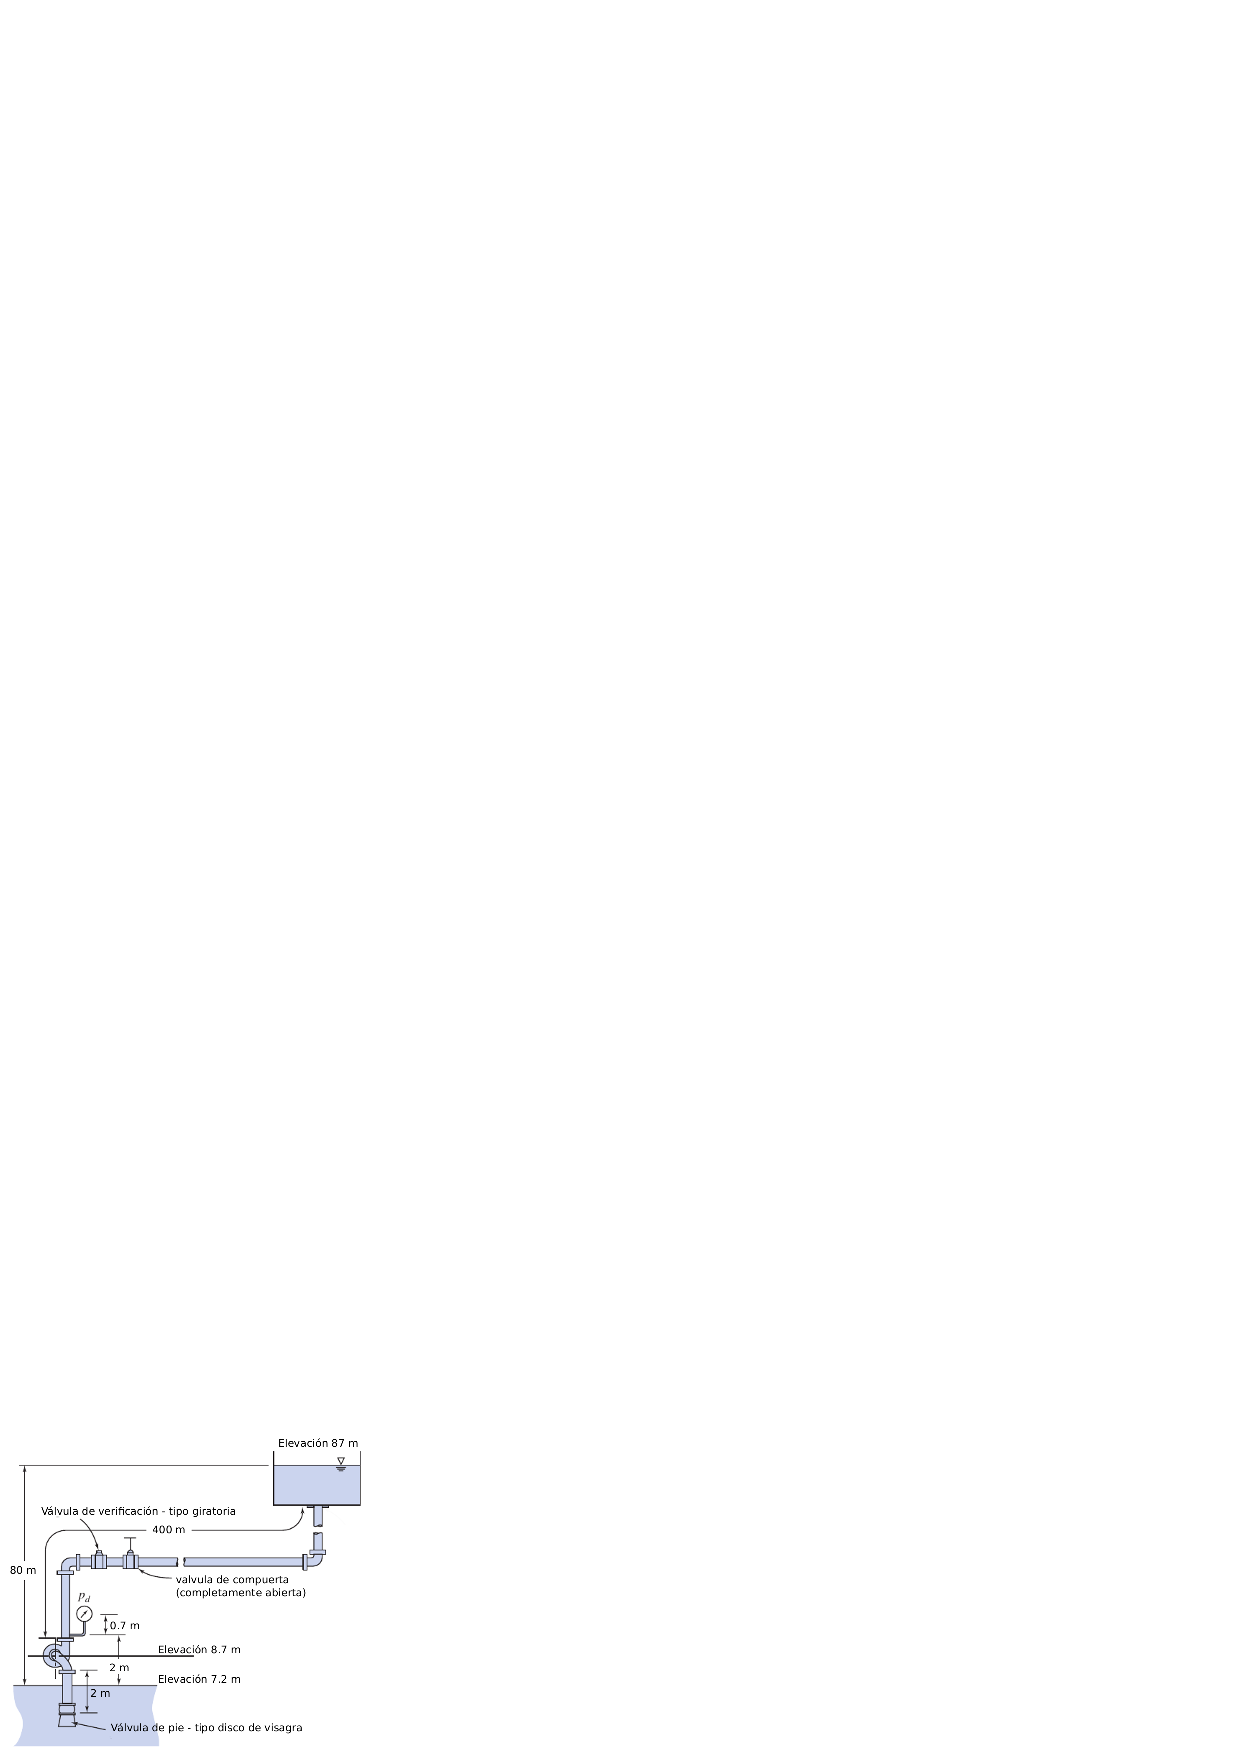
\includegraphics[width=0.4\textwidth]{Figures/p1.png}
\caption{\label{fig:fig1} }
\end{figure}
\columnbreak
\vspace*{\fill}
\begin{figure}[H]
\centering\includegraphics[width=0.5\textwidth]{Figures/p2.png}
\caption{\label{fig:fig2}}
\end{figure}
\end{center}
\end{multicols}

\footnotetext{Pritchard, Philip J. Fox and McDonald’s Introduction to Fluid Mechanics (8th ed.). John Wiley $\&$ Sons. (2011).}

%%%%%%%%%%%%%%%%%%%%%%%%%
\newpage
%%%%%%%%%%%%%%%%%%%%%%%%%
\vspace{1cm}

\underline {Problema 3 (P. 4.65 Fox):}

\vspace{0.2cm}

Calcule la fuerza requerida para mantener el pist\'on en la salida de la tuber\'ia de agua representada en la figura~\ref{fig:fig3}. Considere flujo volum\'etrico de $1.5$\,m$^3$/s y presi\'on aguas arriba de $3.5$\,MPa (abs).

%\begin{figure}[H]
%\centering\includegraphics[width=0.5\textwidth]{Figures/p3.png}
%\caption{\label{fig:fig3}}
%\end{figure}

\begin{figure}[H]
\vfill

\centering\includegraphics[width=0.4\textwidth]{Figures/p3.png}
\caption{\label{fig:fig3} }
\end{figure}

\vspace{1cm}

\underline {Problema 4 (P. 4.72 Fox):}

Una compuerta de $1$\,m de ancho y $1.2$\,m de altura contiene a un cuerpo de agua, tal  como se representa en la figura ~\ref{fig:fig4}. La compuerta est\'a conectada fondo mediante una bisagra. En el lado opuesto al cuerpo de agua, un chorro de agua de $5$\,cm de di\'ametro golpea la compuerta a una altura de $1$\,m. 

\begin{enumerate}[label=\alph*)]
\item ¿Qu\'e velocidad $V$ se requiere para mantener el sistema en equilibrio?.
\item Suponga que el nivel del cuerpo de agua se reduce a $0.5$\,m; ¿Qu\'e velocidad es requerida ahora?
\item Suponga que el nivel de agua se reduce nuevamente, ahora a $0.25$\,m; ¿Qu\'e velocidad es requerida ahora?
\end{enumerate}

\begin{figure}[H]
\centering\includegraphics[width=0.5\textwidth]{Figures/p4.png}
\caption{\label{fig:fig4}}
\end{figure}
%\begin{multicols}{2}
%\begin{center}
%
%\columnbreak
%
%\end{center}
%\end{multicols}
%%
%\begin{figure}[H]
%\centering\includegraphics[width=0.5\textwidth]{Figures/p4.png}
%\caption{\label{fig:fig3}}
%\end{figure}
%%%%%%%%%%%%%%%%%%%%%%%%%
\newpage


\vspace{1cm}

\underline {Problema 5 (P. 6.19 Çengel\footnote{footnotes working fine}):}

Un chorro de agua horizontal de $2.5 \mathrm{~cm}$ de diámetro con una velocidad $V_{j}=40 \mathrm{~m} / \mathrm{s}$ con respecto al suelo es desviado por un cono estacionario de $60^{\circ}$, cuya base tiene un diámetro de 25 cm. La velocidad del agua a lo largo del cono varía linealmente desde cero en la superficie del cono hasta la velocidad del chorro entrante de $40 \mathrm{~m} / \mathrm{s}$ en la superficie libre. Sin tener en cuenta el efecto de la gravedad y las fuerzas cortantes, determine la fuerza horizontal $F$ necesaria para mantener el cono estático.

\begin{figure}[H]
\centering\includegraphics[width=0.5\textwidth]{Figures/p5.png}
\caption{\label{fig:fig5}}
\end{figure}


%
%
%\vspace{1cm}

%\underline {Problema 6 (P. 6.20 Çengel\footnote{footnotes working fine}):}
%
%Se usa un codo de $90^{\circ}$ para dirigir hacia arriba un flujo de agua que viene por un tubo horizontal a razón de $40 \mathrm{~kg} / \mathrm{s}$. El diámetro del codo en toda su longitud es de $10 \mathrm{~cm}$. Dicho codo descarga el agua hacia la atmósfera y, por lo tanto, la presión a la salida es la presión atmosférica local. La diferencia de elevación entre los centros de la salida y de la entrada del codo es de $50 \mathrm{~cm}$. Se considera que el peso de este codo y del agua que está en él es despreciable. Determine $a$ ) la presión manométrica en el centro de la entrada del codo y $b$ ) la fuerza de anclaje necesaria para mantener el codo en su sitio. Tome el factor de corrección del flujo de la cantidad de movimiento como $1.03$ tanto a la entrada como a la salida.
%
%
%
%\begin{figure}[H]
%\centering\includegraphics[width=0.4\textwidth]{Figures/p6.png}
%\caption{\label{fig:fig6}}
%\end{figure} 
%\footnotetext{Yunus A. Çengel, John M. Cimbala. Mecánica de fluidos: Fundamentos y aplicaciones 4/e. McGraw-Hill , 2018.}

%%%%%%%%%%%%%%%%%%%%%%%%%
%%%%%%%%%%%%%%%%%%%%%%%%%
%%%%%%%%%%%%%%%%%%%%%%%%%
\end{document}
